%%%%%%%%%%%%%%%%%%%%%%%%%%%%%%%%%%%%%%%%%%%%%%%%%%%%%%%%%%%%%%%%%%%%%%%%%%%%%%%%%%
\begin{frame}[fragile]\frametitle{}
\begin{center}
{\Large Conclusions}
\end{center}
\end{frame}

%%%%%%%%%%%%%%%%%%%%%%%%%%%%%%%%%%%%%%%%%%%%%%%%%%%%%%%%%%%
\begin{frame}[fragile]\frametitle{So, What is RAG?}

\begin{itemize}
\item A new paradigm for generation tasks, combining retrieval and generation models.
\item Motivation: Overcoming limitations of pure generative models in factual consistency, efficiency, and diversity.
\item Impact: Improved performance in text summarization, question answering, and other NLP tasks.
\end{itemize}	

\end{frame}


%%%%%%%%%%%%%%%%%%%%%%%%%%%%%%%%%%%%%%%%%%%%%%%%%%%%%%%%%%%
\begin{frame}[fragile]\frametitle{RAG Architecture}


		\begin{center}
		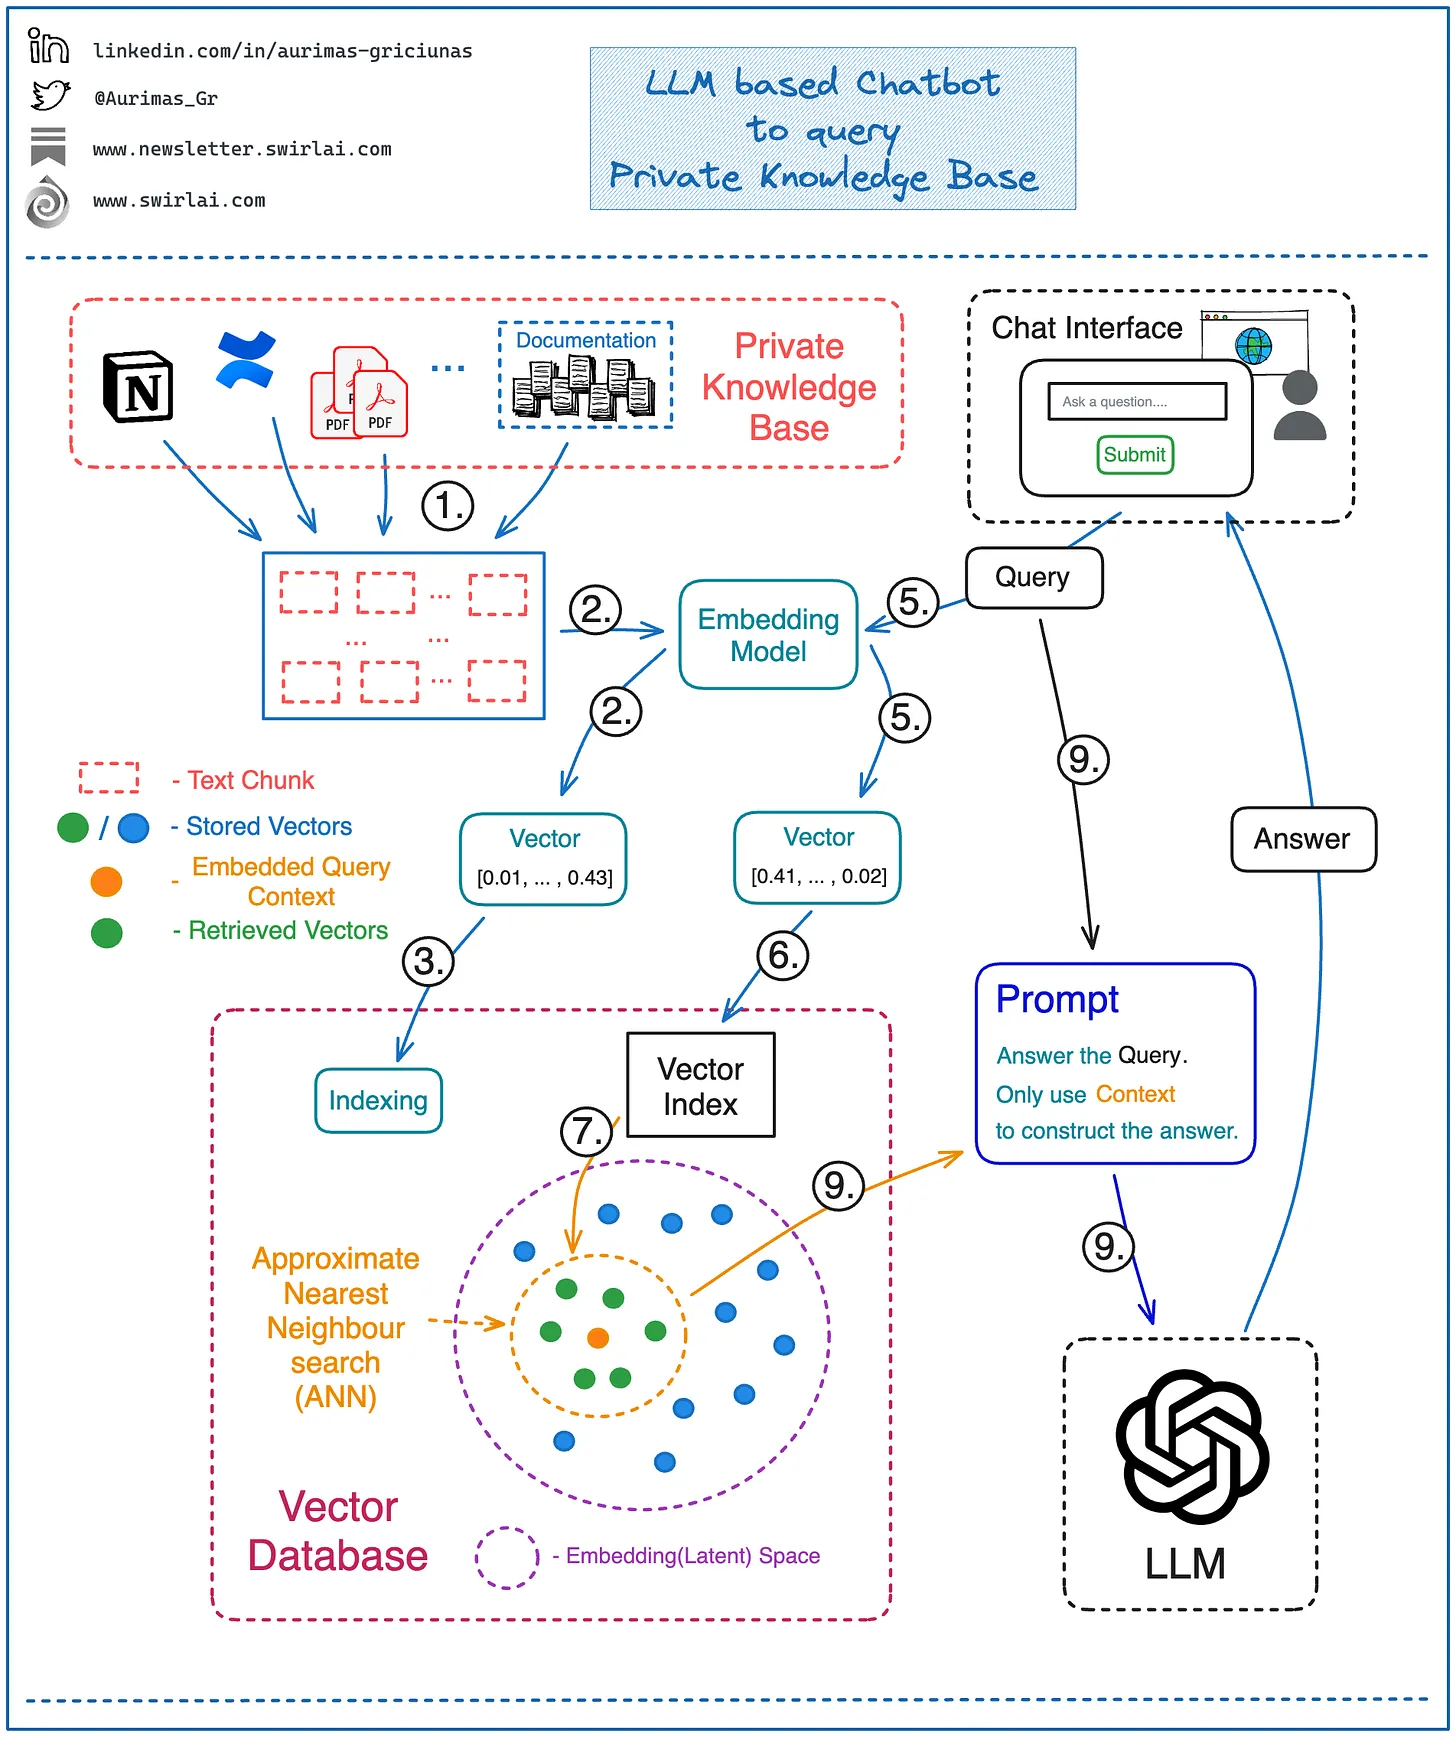
\includegraphics[width=0.5\linewidth,keepaspectratio]{chatgpt47}
		\end{center}

{\tiny (Ref: Overview of Large Language Models - Aman AI)}

\end{frame}


%%%%%%%%%%%%%%%%%%%%%%%%%%%%%%%%%%%%%%%%%%%%%%%%%%%%%%%%%%%
\begin{frame}[fragile]\frametitle{RAG Architecture}

\begin{itemize}
  \item \textbf{Powerful Enhancement:}
    \begin{itemize}
      \item RAG provides additional memory and context.
      \item Increases confidence in LLM responses.
    \end{itemize}

  \item \textbf{Architecture:}
    \begin{itemize}
      \item Two essential pipelines for an effective RAG system.
    \end{itemize}
  
  \item \textbf{Indexing Pipeline:}
    \begin{itemize}
      \item Retrieves knowledge from diverse sources.
      \item Enables loading, splitting, and embedding creation for offline use.
      \item Can be on-the-fly for lower volume and single-use scenarios.
    \end{itemize}

  \item \textbf{Generation Pipeline:}
    \begin{itemize}
      \item Retriever fetches information from the knowledge base.
      \item Retrieved data augments user prompt and is sent to the LLM.
      \item LLM generates text and sends the response back to the user.
    \end{itemize}

  \item \textbf{Evaluation Pipeline:}
    \begin{itemize}
      \item Optional pipeline for assessing groundedness and relevance of responses.
    \end{itemize}
\end{itemize}

{\tiny (Ref: RAG Architecture -Abhinav  Kimothi)}

\end{frame}

%%%%%%%%%%%%%%%%%%%%%%%%%%%%%%%%%%%%%%%%%%%%%%%%%%%%%%%%%%%
\begin{frame}[fragile]\frametitle{Challenges and Future Directions}

\begin{itemize}
\item Bias Mitigation: Addressing potential biases introduced by the retrieval component.
\item Domain Adaptation: Adapting RAG models to specific domains with limited training data.
\item Interpretability Enhancement: Understanding the reasoning behind generated outputs for better model debugging.
\end{itemize}	

\end{frame}